\documentclass[serif,9pt]{beamer}
\usetheme{tree}

\usepackage[latin1]{inputenc}
\usepackage[spanish]{babel}
\usepackage{caption}
\usepackage{graphicx} % figuras
\usepackage{subfigure} % subfiguras
\usepackage{float}

\restylefloat{figure}

\beamersetuncovermixins{\opaqueness<1>{25}}{\opaqueness<2->{15}}

\AtBeginSection[]
{
  \begin{frame}<beamer>{Contenido}
    \tableofcontents[currentsection]
  \end{frame}
}

\AtBeginSubsection[]
{
  \begin{frame}<beamer>{Contenido}
    \tableofcontents[currentsection,currentsubsection]
  \end{frame}
}

\begin{document}

\title{Pr�ctica 2: Algoritmos Divide y Vencer�s}  
\author{David Cabezas Berrido}
\date{}

\begin{frame}
\titlepage
\end{frame}

\begin{frame}{Contenido}
\tableofcontents
\end{frame} 

\section{Algoritmo ``obvio''}

\begin{frame}[fragile]{Algoritmo ``obvio''}
\begin{verbatim}
    1  int enSuPosicion(int* T, int n){
    2    int i = -1, j;
    3    bool found = false;
    4  
    5    for(j = 0; j < n && !found; j++){
    6      if(T[j] == j){
    7        i = j;
    8        found = true;
    9      }
   10    }
   11  
   12    return i;
   13  }
\end{verbatim}
\end{frame}

\begin{frame}{Ajuste del algoritmo ``obvio''}
\begin{figure}[H]
  \centering
  \label{}
  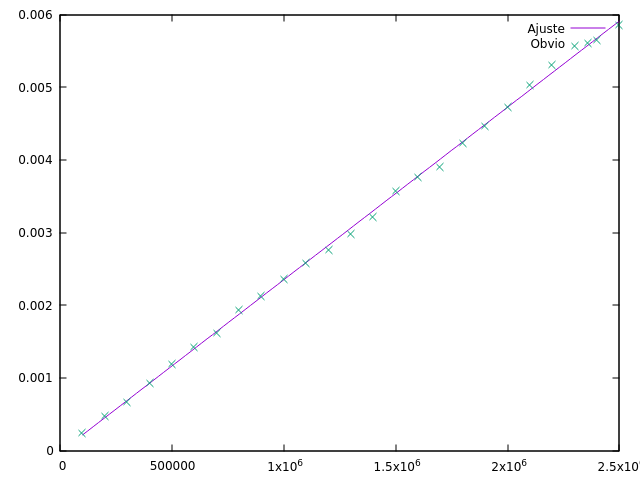
\includegraphics[width=75mm]{graficos/ajusteObvio}
\end{figure}
\vspace{-7mm}
  \[f(x)=2.37482\mbox{e}-09x-2.47917\mbox{e}-05\]
  \[\mbox{RMS}=5.83941\mbox{e}-05\]
\end{frame}

\section{Primer caso: Todos los elementos son diferentes}

\begin{frame}[fragile]{Algoritmo DyV}
\begin{verbatim}
    1  int enSuPosicion(int *T, int n){
    2    
    3    int result=-1, left=0, right=n-1;
    4    int p = (left+right)/2;
    5    bool found = false;
    6    
    7    while(!found and left <= right){
    8      if(p == T[p]){
    9        result = p;
   10        found = true;
   11      } else if(p < T[p])
   12        right = p-1;
   13      else
   14        left = p+1;
   15  
   16      p = (left+right)/2;
   17    }
   18    return result;
   19  }
\end{verbatim}
\end{frame}

\begin{frame}{Algoritmo DyV frente al ``obvio''}
\begin{figure}[H]
  \centering
  \label{}
  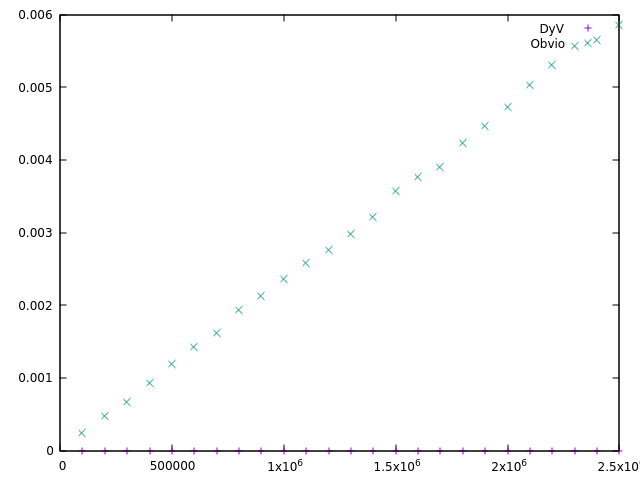
\includegraphics[width=90mm]{graficos/comparacion}
\end{figure}
\end{frame}

\begin{frame}{Ajuste del algoritmo DyV}
\begin{figure}[H]
  \centering
  \label{}
  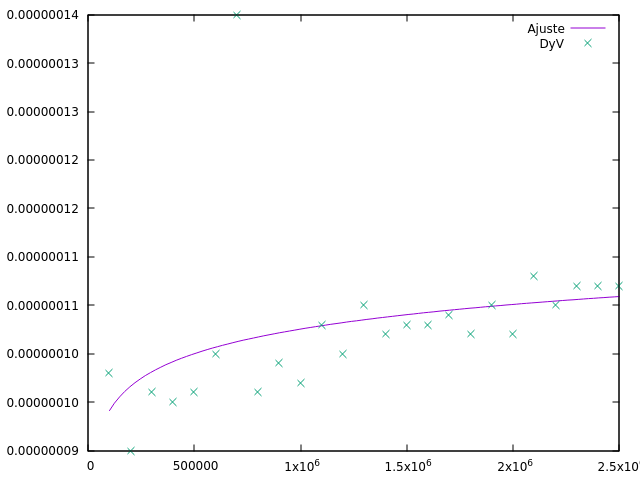
\includegraphics[width=75mm]{graficos/ajusteDyV}
\end{figure}
\vspace{-7mm}
  \[f(x)=3.66877\mbox{e}-09\log(0.975496x+1)+5.19407\mbox{e}-08\]
  \[\mbox{RMS}=8.04501\mbox{e}-09\]
\end{frame}

\section{Segundo caso: Se repiten elementos}

\begin{frame}[fragile]{Algoritmo DyV}
\begin{verbatim}
    1  int enSuPosicionLims(int *T, int l, int r){
    2
    3    if(r <= l) return -1;
    4    
    5    int p = (l+r-1)/2;
    6    if(p == T[p]) return p;
    7  
    8    int res;
    9    if(p < T[p]){
   10      if((res = enSuPosicionLims(T, l, p)) != -1)
   11        return res;
   12  
   13      return enSuPosicionLims(T, T[p], r);
   14    }
   15    if((res = enSuPosicionLims(T, p+1, r)) != -1)
   16      return res;
   17        
   18    return enSuPosicionLims(T, l, T[p]+1);
   19  }
\end{verbatim}
\end{frame}

\begin{frame}{Algoritmo DyV frente al ``obvio''}
\begin{figure}[H]
  \centering
  \label{}
  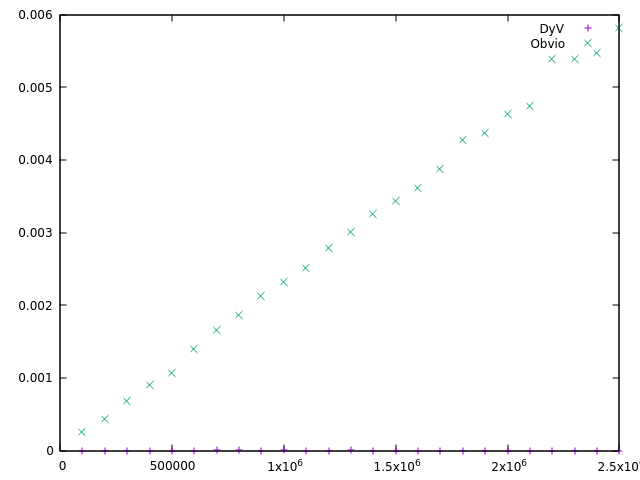
\includegraphics[width=90mm]{graficos/comparacion_Repetidos}
\end{figure}
\end{frame}

\begin{frame}{Ajuste del algoritmo DyV}
\begin{figure}[H]
  \centering
  \label{}
  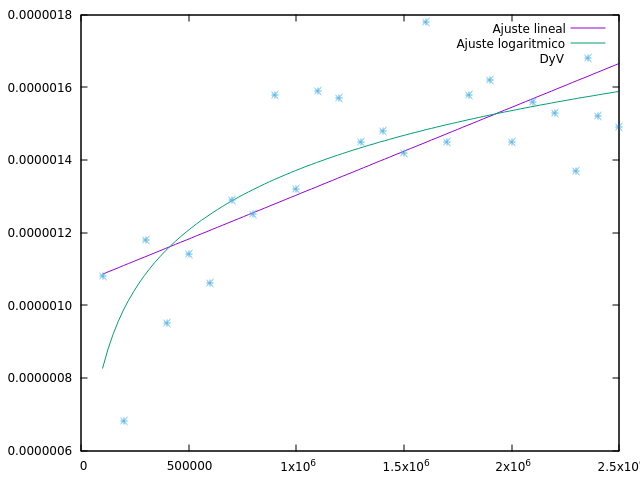
\includegraphics[width=90mm]{graficos/ajustes-rep}
\end{figure}
\end{frame}

\begin{frame}{Ajuste del algoritmo DyV}
  Ajuste por funci�n lineal:
  \[f(x) = 2.41769 \mbox{e} -13x + 1.0613 \mbox{e} -06\]
  \[\mbox{RMS}=1.77413\mbox{e}-07\]
  
  \vspace{7mm}

  Ajuste por funci�n logar�tmica:
  \[g(x) = 2.37005 \mbox{e} -07\log(0.975496x+1)-1.89703 \mbox{e} -06\]
  \[\mbox{RMS}=1.61174\mbox{e}-07\]
\end{frame}

\section{�Son los ejemplos adecuados?}

\subsection{Alternativa al algoritmo obvio: Problema del ajuste}

\begin{frame}[fragile]{Algoritmo ``obvio'' inverso}
\begin{verbatim}
    1  int enSuPosicion(int* T, int n){
    2    int i = -1, j;
    3    bool found = false;
    4  
    5    for(j = n-1; j >=0 && !found; j--){
    6      if(T[j] == j){
    7        i = j;
    8        found = true;
    9      }
   10    }
   11  
   12    return i;
   13  }
\end{verbatim}
\end{frame}

\begin{frame}{Ajuste del algoritmo ``obvio'' hacia atr�s}
  \begin{figure}[H]
  \centering
  \caption*{Todos los elementos son distintos}
  \label{}
  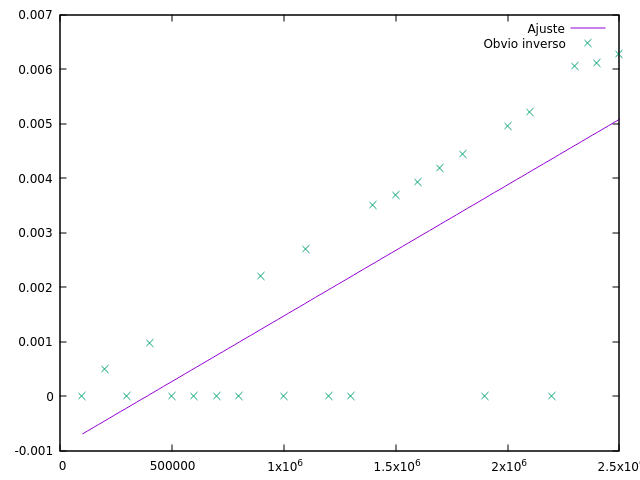
\includegraphics[width=75mm]{graficos/ajuste_obvio-inverso-distintos}
\end{figure}
\vspace{-7mm}
\[f(x)=2.40612\mbox{e}-09x-0.000937639\]
\[\mbox{RMS}=0.0016428\]
\end{frame}

\begin{frame}{Ajuste del algoritmo ``obvio'' hacia atr�s}
  \begin{figure}[H]
  \centering
  \caption*{Hay elementos repetidos}
  \label{}
  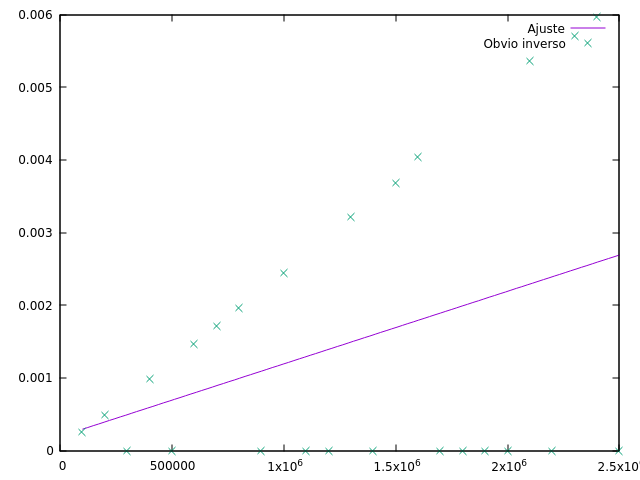
\includegraphics[width=75mm]{graficos/ajuste_obvio-inverso-repetidos}
\end{figure}
\vspace{-7mm}
\[f(x)=9.99324\mbox{e}-10+0.000192786\]
\[\mbox{RMS}=0.00191864\]
\end{frame}

\subsection{Soluci�n: Multiples mediciones}

\begin{frame}{Ajuste del algoritmo ``obvio'' hacia atr�s}
  \begin{figure}[H]
  \centering
  \caption*{Todos los elementos son distintos}
  \label{}
  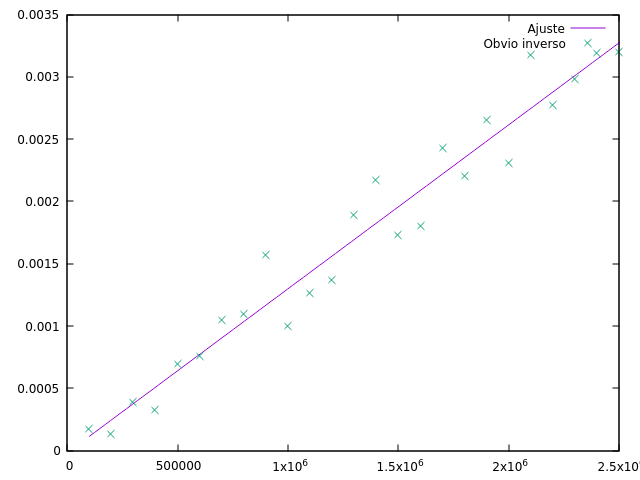
\includegraphics[width=75mm]{graficos/ajust-sol-dist}
\end{figure}
\vspace{-7mm}
\[f(x)=1.31781\mbox{e}-09x-1.9522e-05\]
\[\mbox{RMS}=0.00021679\]
\end{frame}

\begin{frame}{Ajuste del algoritmo ``obvio'' hacia atr�s}
  \begin{figure}[H]
  \centering
  \caption*{Hay elementos repetidos}
  \label{}
  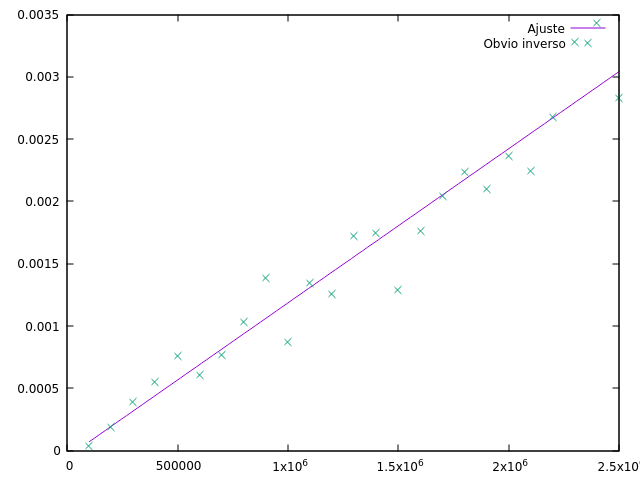
\includegraphics[width=75mm]{graficos/ajust-sol-rep}
\end{figure}
\vspace{-7mm}
\[f(x)=1.23924\mbox{e}-09-5.40427e-05\]
\[\mbox{RMS}=0.000239843\]
\end{frame}

\end{document}